\documentclass{sig-alternate-05-2015}

\usepackage{graphicx}
\usepackage{multicol}
\usepackage{multirow}

\begin{document}

% Copyright
\setcopyright{acmcopyright}
%\setcopyright{acmlicensed}
%\setcopyright{rightsretained}
%\setcopyright{usgov}
%\setcopyright{usgovmixed}
%\setcopyright{cagov}
%\setcopyright{cagovmixed}



% DOI
\doi{10.475/123_4}

% ISBN
\isbn{123-4567-24-567/08/06}

%Conference
\conferenceinfo{PLDI '13}{June 16--19, 2013, Seattle, WA, USA}

\acmPrice{\$15.00}

%
% --- Author Metadata here ---
\conferenceinfo{WOODSTOCK}{'97 El Paso, Texas USA}
%\CopyrightYear{2007} % Allows default copyright year (20XX) to be over-ridden - IF NEED BE.
%\crdata{0-12345-67-8/90/01}  % Allows default copyright data (0-89791-88-6/97/05) to be over-ridden - IF NEED BE.
% --- End of Author Metadata ---

\title{API Recognition in StackOverflow Posts}

%
% You need the command \numberofauthors to handle the 'placement
% and alignment' of the authors beneath the title.
%
% For aesthetic reasons, we recommend 'three authors at a time'
% i.e. three 'name/affiliation blocks' be placed beneath the title.
%
% NOTE: You are NOT restricted in how many 'rows' of
% "name/affiliations" may appear. We just ask that you restrict
% the number of 'columns' to three.
%
% Because of the available 'opening page real-estate'
% we ask you to refrain from putting more than six authors
% (two rows with three columns) beneath the article title.
% More than six makes the first-page appear very cluttered indeed.
%
% Use the \alignauthor commands to handle the names
% and affiliations for an 'aesthetic maximum' of six authors.
% Add names, affiliations, addresses for
% the seventh etc. author(s) as the argument for the
% \additionalauthors command.
% These 'additional authors' will be output/set for you
% without further effort on your part as the last section in
% the body of your article BEFORE References or any Appendices.

\numberofauthors{4} %  in this sample file, there are a *total*
% of EIGHT authors. SIX appear on the 'first-page' (for formatting
% reasons) and the remaining two appear in the \additionalauthors section.
%
\author{
% You can go ahead and credit any number of authors here,
% e.g. one 'row of three' or two rows (consisting of one row of three
% and a second row of one, two or three).
%
% The command \alignauthor (no curly braces needed) should
% precede each author name, affiliation/snail-mail address and
% e-mail address. Additionally, tag each line of
% affiliation/address with \affaddr, and tag the
% e-mail address with \email.
%
% 1st. author
\alignauthor
Madhavan Seshadri\\
       \affaddr{School of Computer Engineering}\\
       \affaddr{Nanyang Technological University}\\
       \affaddr{Singapore}\\
       \email{madhavan001@ntu.edu.sg}
\alignauthor  
Sanjana Jayakymar\\
       \affaddr{School of Computer Engineering}\\
       \affaddr{Nanyang Technological University}\\
       \affaddr{Singapore}\\
       \email{sanjana002@ntu.edu.sg}
\alignauthor
Ankur Bansal\\
       \affaddr{School of Computer Engineering}\\
       \affaddr{Nanyang Technological University}\\
       \affaddr{Singapore}\\
       \email{ankur005@ntu.edu.sg}\\
\and
\alignauthor
Mohit Gambani Gurno\\
       \affaddr{School of Computer Engineering}\\
       \affaddr{Nanyang Technological University}\\
       \affaddr{Singapore}\\
       \email{gamb0002@ntu.edu.sg}\\       
}

\maketitle
\begin{abstract}
With a user base of over 4,000,000, Stack Overflow is a popular online forum for programmers to share their knowledge by discussing a diverse range of topics in computer programming. The purpose of this project was to develop a model to recognize the APIs mentioned by users, in their posts, on Stack Overflow. The process of building the model consisted of three progressive stages. The first stage involved collection and pre-processing of data, in the form of user posts, from Stack Overflow. The second stage dealt with manually annotating the API mentions in the previously obtained dataset. The annotated data was further fed into a Conditional Random Field (CRF) classifier, which used named entity recognition, to come up with a model to recognize API mentions, as part of the final stage. The effectiveness of the model was then validated using $k-fold$ cross validation process. This validation methodology was repeated with different values of $k$ in a measure to identify the performance over the granularity of the training and validation sets. This has shown a considerable change in Recall values while increasing the number of folds. The potential application of this model and the challenges associated with it were discussed before finally suggesting improved prediction models for the same process. 
\end{abstract}



%
%  Use this command to print the description
%
%\printccsdesc

% We no longer use \terms command
%\terms{Theory}

\keywords{Named Entity Recognition, Conditional random field, API Recognition, Parts of Speech Tagging, Pattern Recognition}

\section{Introduction}
With a total of over 10,000,000 questions posted by users, Stack Overflow has become the go-to online community for programmers worldwide. Since the website caters to questions on a diverse range of topics in computer programming, there are often user posts mentioning APIs, either as part of a code snippet, or just in the middle of a sentence, like “How many spaces will Java String.trim() remove?”. With large amounts of data coming from a comparably large number of sources, and the inconsistencies exhibited by humans, with regards to language, semantics and grammar, when it comes to posting online, it can be especially hard to build a generic model that can accurately identify API mentions in user posts. The later sections of this report elaborate the model building process in detail, and consequently give a verdict on the model’s effectiveness, accounting for attributes such as accuracy, precision, recall and f-measure. Finally, there is a section identifying how the recognized results can be used in applications to make programmers’ life better, followed by conclusion and references.



\section{Literature Review}
The API recognition problem can be treated akin to a Proper Name detection problem, which is a widely studied domain in the field of Natural Language Processing. Several approaches can be taken for the detection of proper names within a sequence of tokens.
The API recognition problem can be regarded as a pattern recognition problem or a simple classification problem, (where the set of tokens can be classified as an API or not) or a Named Entity Recognition \cite{grishman1996message} Problem (which uses the context of the sequence of words appearing in the text and treats them as named entities).

\subsection{Proper Name Detection}
In the proper name detection, the similarity measures are typically used for the detection and search of the proper names. Typically, the known similarity measures deal with phonetic similarity, typing errors and plain string similarity. All these similarity measures are known to achieve significantly higher retrieval quality than the normal plain identity. \cite{pfeifer1996retrieval}

There have been several studies and experiments performed such as those to automatically detect and retrieve proper names from Non-Journalistic Texts \cite{poibeau2001proper}. However, such studies are very specific and use the same approach as the detection of Proper Names as used in Journalistic Texts by proposing measures to account and cater the differences among a Journalistic and Non-Journalistic text (limiting to formal modes of communication such as emails).

Another popular study in this domain is the Identification of Proper names studied in \cite{fukuda1998toward} where the authors use the surface clue on the strings to obtain a pattern for the protein naming. The main advantage of such an approach is that it could detect protein names which could be an author generated content. However, this naming takes advantage of the naming conventions followed for naming a protein which may not always be the same case for API recognition as naming conventions differ according to the coding language of the StackOverflow post and variation of naming in proteins is little depending upon its constituents.

Such approaches cannot be used for API recognition, primarily due to the following reasons: 1.The API mentions may not necessarily be in the same context (sequence of tokens) as a proper name mention as studied in the previous approaches. 2. The language used by the users in StackOverflow posts may not be journalistic/formal in nature.

\subsection{Named Entity Recognition}
As explained earlier, the task of recognizing API mentions among a series of posts is a classic named entity recognition problem. Since the classification of API's is a relatively new problem in the domain of Natural Language processing, much of the prior studies have been in the domain of Named Entity Recognition which can be studied upon meticulously for the project. A typical named entity recognition problem can be categorized into two parts, namely Entity Recognition (which is the recognition of names as entities) and classification of these entities\cite{tjong2003introduction}.

One of the major advantage of a named Entity Recognition model is the ability to detect previously unrecognised 'Entity' based on the supervised and semi-supervised learning performed during the training phase of the model.

Supervised learning phase of an NER model consists of a system that reads large annotated corpus, memorizes the annotated entities, and creates a list of dis-ambiguous rules based on the discriminative features. Several such techniques have been studied over the last 20 years, such as HMM model \cite{bickel1998efficient},  Support Vector Machines(SVMs) \cite{asahara2003japanese} which was used in Japanese Named Entity Extraction, Conditional Random Fields \cite{okanohara2006improving} etc.

In a semi-supervised learning approach, the Named Entity Recognition system first takes a corpus as input and obtains contextual clues based on this input data. So when a new input text is presented to this model, the rules previously derived are then applied for recognition of new names. The learning process is then re-applied to the whole set in the aim of generating new contextual rules. Several approaches of semi-supervised learning used are Regular-expression matching \cite{brin2012reprint} for web crawling (however the pattern of web URL naming is fixed), Multi-level bootstrapping technique to alternatively select the best extraction pattern and bootstrap its extraction into the corpus. This process retains only the most reliable entries in the corpus \cite{riloff1999learning}.


\subsection{Studies on StackOverflow Posts}
Several studies have been made on the data pertaining to the individual posts in StackOverflow. Several of them include, \cite{stanley2013predicting} which established a methodology for predicting the tags associated with each of the posts. The paper presents a Bayesian Regression based model for predicting the tags associated with the posts. The study opens up new possibilities for the API recognition problem itself. Under the assumption that the API's of different languages are significantly different among themselves, this approach of predicting the missing tags and then studying all the possible combinations by using an ensemble may theoretically result in a better accuracy for the NER model with the training parameters being different among the ensembles. Though it is a good solution for the problem, we are not implementing the same for the scope of this project and is potentially a future research topic.

There have also been studies such as \cite{bazelli2013personality} which is helpful in outlining the characteristics of the different users.

\begin{figure}
\centering
  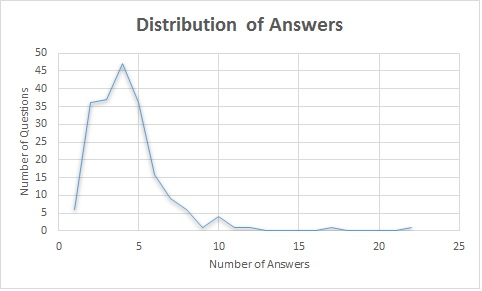
\includegraphics[width=0.75\linewidth]{AnswerDistribution.jpg}
  \caption{Distribution of Answers}
  \label{fig:distribution}
\end{figure}

\begin{figure}
\centering
  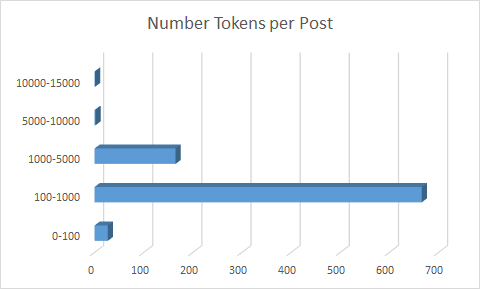
\includegraphics[width=0.75\linewidth]{NumberTokens.png}
  \caption{Bar Graph: Number of Tokens in the range}
  \label{fig:tokens}
\end{figure}

\section{Dataset Generation}
The following subsections were performed for obtaining a clean and relevant data pertaining to the problem as per the requirements of this assignment. The main source of data is the StackOverflow Dump available online. The dataset itself is an xml file and each element in this xml file corresponds to one post generated by the user. A post may be a question or an answer with the questions being tagged with different languages. Example of such tags are (C++,JAVA,C). The data dump file used for this project was obtained from \cite{stackexchange} which contains all the posts and its information as an xml file.

\subsection{Extraction of relevant posts}
The dataset which was obtained from the Stack Exchange website was then pre-processed as per the requirements of this project which is to process a dataset of more than 500 posts in total which has atleast 100 posts with API mentions. The definition of post as mentioned is either a question or an answer. From the large set of posts, to reduce the complexity of identifying the API's only the questions with tags matching any of (JAVA, C++, Python, API, String) were chosen. From the chosen posts, manual marking of a posts with a valid API was done to ensure that the dataset contains atleast 100 such posts.

\subsection{Tokenization}
The process of tokenization is the process of converting text into smaller linguistic units such as words, punctuations, numbers etc. In this project, the posts were converted into a smaller set of tokens using nltk.tokenize() function available from the nltk library\cite{bird2006nltk} for further processing.

\subsection{Dataset Analysis}
The total number of posts were 863 and the number of questions were 201 and the answers associated with these questions were 662 posts in number.
\subsubsection{Answers per question}
Figure \ref{fig:distribution} shows the distribution of the number of Questions vs. number of Answers. The mode of the number of answers in the dataset was 3. The number of answers per question spanned from 0 and upto 21 in the dataset. Only 1 question had a maximum number of answers as 21.

\subsubsection{Number of tokens}
The number of tokens per post(questions \& answers) has a range from 26 to 14670. Figure \ref{fig:tokens} is the distribution of the number of tokens and the corresponding number of posts. The number of posts in the range of 5000-10000 and 10000-15000 are 2 and 1 respectively. The range 100-1000 has the mode of 666.

\section{Dataset Analysis}
The following section is used to analyze the dataset and prepare the same to be processed in the next step. The section consists of three parts, namely stemming, Parts-of-Speech Tagging and API Annotation.

\subsection{Stemming}
Stemming is an important pre-processing step in  many applications of NLP. The main goal of stemming is to reduce the number of inflectional or derivational forms of words thereby reducing the memory required for storing each of them. An alternative to the process of Stemming would be 'Lemmatization' which provides morphological analysis to get the lemma of each word. A complete morphological analysis for the whole data is known to give very low benefits to the process of retrieval. As such, a stemmer helps in the reduction of space complexity for the application which are built on top of it. For the purpose of the project itself, Porter's stemming\cite{porter1980algorithm} was used which removes all the suffixes from the words to produce a stem of it. A typical example of the same is 'Lemmatization' will be stemmed to 'Lemma'.

Figure \ref{fig:beforeRemovingStopWords} shows the change in the list of top 20 words before the stop words are removed. As such, since the stop words generally do not appear as a stem of other words, the effect of the change in this list is minimal as most of the stop words remain, however the notable changes are the appearance of words \{use\} and the rise in the number of occurrences of \{have, do\} as these words form the stem of several other words such as \{having, had, does, doing\}.

Figure \ref{fig:afterRemovingStopWords} shows a significant change in the list of top 20 words when the stemming is performed after the removal of stop words. The most notable change is the increase in number of occurrences of \{use\} which is the stem word for both \{use, using\} among others.The top two words in the list combine to form a unified one. Other notable differences are the increase in occurrence of \{get, work, method\} in the second list among others and also the disappearance of \{data\} which has no stemmed word.
\begin{figure}
\centering
  \raisebox{-0.5\height}{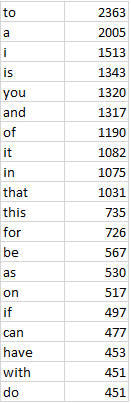
\includegraphics[width=0.3\linewidth]{BStemmingBStopWords.png}}
  \centering
  \raisebox{-0.5\height}{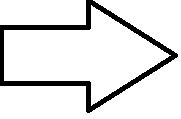
\includegraphics[width=0.30\linewidth]{rightArrow.png}}
  \raisebox{-0.5\height}{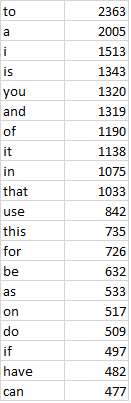
\includegraphics[width=0.30\linewidth]{AStemmingBStopWords.png}}
  \caption{Effect of Stemming before removing stop words}
  \label{fig:beforeRemovingStopWords}
\end{figure}

\begin{figure}
\centering
  \raisebox{-0.5\height}{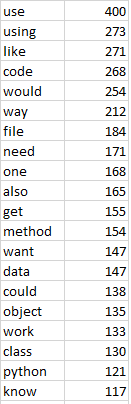
\includegraphics[width=0.3\linewidth]{BStemmingAStopWords.png}}
  \centering
  \raisebox{-0.5\height}{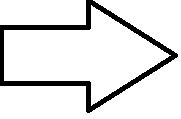
\includegraphics[width=0.30\linewidth]{rightArrow.png}}
  \raisebox{-0.5\height}{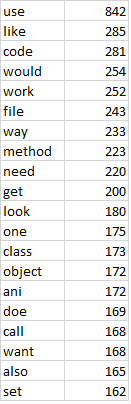
\includegraphics[width=0.30\linewidth]{AStemmingAStopWords.png}}
  \caption{Effect of Stemming after removing stop words}
  \label{fig:afterRemovingStopWords}
\end{figure}

\subsection{POS Tagging}

As a prerequisite of the assignment, 10 sentences from the dataset collected earlier were selected. Each sentence was chosen in a manner such that it contains an API mention. For each of the selected sentences, manual POS tagging was implemented. The results of the tags are as shown below: 

\begin{description}
\item[1.]
You would use a List to store a list of student details in a class \linebreak
{[You/Pronoun]} [would/Verb] [use/Verb] [a/Determiner] \linebreak
{[List/Noun]}{[to/Preposition]} [store/Verb] [a/Determiner] \linebreak
{[list/Noun]}{[of/Preposition]}[student/Noun][details/Noun] \linebreak
{[in/Preposition]}{[a/Determiner]} [class/Noun]

\item[2.]
Request.Form only includes variables posted through a form \linebreak
{[Request.Form/Noun]} [only/Adverb] [includes/Verb] \linebreak
{[variables/Noun]}[posted/Verb] [through/Preposition] \linebreak
{[a/Determiner]} [form/Noun]

\item[3.]
Request.Params includes both posted form variables and get variables specified as URL parameters. \linebreak
{[Request.Params/Noun]} [includes/Verb] \linebreak
{[both/Determiner]} {[posted/Verb]}[form/Noun] \linebreak
{[variables/verb]} [and/Conjunction]{[get/Verb]} \linebreak
{[variables/Noun]}[specified/Verb] [as/Preposition]\linebreak
{[URL/Noun]} [parameters/Noun]

\item[4.]
If Array.Length were unsigned, and added to a negative int there could be messy results. \linebreak
{[If/Preposition]} [Array.Length/Noun] [were/Verb] \linebreak
{[unsigned/Adjective]}, {[and/Conjunction]} [added/Verb] \linebreak
{[to/Preposition]} {[a/Determiner]} [negative/Adjective] \linebreak
{[int/Noun]} [there/Determiner] [could/Verb] [be/Verb] \linebreak
{[messy/Adjective]} [results/Noun]

\item[5.]
You also delay full parsing and only get additional detail when you call expandNode() \linebreak
{[You/Pronoun]} [also/Adverb] [delay/Verb] \linebreak 
{[full/Adjective]}{[parsing/verb]} {[and/Conjunction]}\linebreak
{ [only/Adverb]} [get/Verb] {[additional/Adjective]} \linebreak
{[detail/Noun]} [when/Adverb] {[you/Pronoun]} \linebreak
{[call/Verb]} [expandNode()/Noun]

\item[6.]
The minidom module, part of the Python Standard Library, will likely suit your needs \linebreak
{[The/Determiner]} [minidom/Noun] [module/Noun] , \linebreak
{[part/Noun]}{[of/Preposition]} [the/Determiner] \linebreak
{[Python/Noun]}{[Standard/Noun]}{[Library/Noun]} ,\linebreak
{[will/Verb]} [likely/Adverb] [suit/Verb] \linebreak
{[your/Pronoun]} [needs/Noun]


\item[7.]
Pass the authority along to an object like a QTextEdit to do the manipulation \linebreak
{[Pass/Verb]} [the/Determiner] [authority/Noun] \linebreak
{[along/Preposition]} [to/Preposition] [an/Determiner] \linebreak
{[object/Noun]} [like/Preposition] [a/Determiner] \linebreak
{[QTextEdit/Noun]} [to/Preposition] [do/Verb] \linebreak
{[the/Determiner]} [manipulation/Noun]

\item[8.]
I believe you could do this by using this.Master.FindControl or something similar \linebreak
{[I/Pronoun]} [believe/Verb] [you/Pronoun] [could/Verb] \linebreak
{[do/Verb]} [this/Determiner] [by/Preposition] \linebreak
{[using/Verb]} [this.Master.FindControl/Noun] \linebreak
{[or/Conjunction]}[something/Noun] [similar/Adjective]

\item[9.]
You could also make an array of c.Name data and use String.Join method to create your line \linebreak
{[You/Pronoun]} [could/Verb] [also/Adverb] [make/Verb]\linebreak
{[an/Determiner]} [array/Noun] [of/Preposition]\linebreak
{[c.Name/Noun]} [data/Noun] [and/Conjunction] \linebreak
{[use/Verb]} [String.Join/Noun] [method/Noun] \linebreak
{[to/Preposition]} [create/Verb] [your/Pronoun] [line/Noun].

\item[10.]
This might not be as performant as the StringBuilder approach, but it definitely looks cleaner \linebreak
{[This/Determiner]} [might/Verb] [not/Adverb] [be/Verb] \linebreak
{[as/Preposition]} [performant/Adjective] [as/Preposition] \linebreak
{[the/Determiner]} [StringBuilder/Noun] [approach/Noun], \linebreak
{[but/Conjunction]} [it/Pronoun] [definitely/Adverb] \linebreak
{[looks/Verb]} [cleaner/Adjective].
\end{description}

It can be seen from the process above that all API mentions are considered to be Noun terms. These terms are generally followed by Determiners or Verbs. We have utilized the basic parts of speech that is commonly used in English - noun, verb, adjective, preposition, pronoun, adverb, conjunction, and determiner.

\subsection{API Annotation}
As mentioned earlier, the posts retrieved through crawling and cleaning within our dataset contains many API mentions. As a requirement of the assignment, a sample of 100 posts were to be annotated, each post containing at least one API mention. In order to do so, a specific definition of an API was devised. 

\subsubsection{Definition of API}
In order to commence the process of annotation, an appropriate definition of an API mention was required. Posts under the category of common programming languages are retrieved. Within these posts, parts of code within the <code></code> tags are specifically considered to contain API mentions. These could be classes, function calls – both user defined and built-in, or specific libraries and softwares that are commonly used. Code appearing in the {<pre><code>}\linebreak
{</code></pre>} tags are not considered as these are majorly code blocks. The definition is restricted to API mentions within the post description, rather than in the code block. 


The format of a function call is confined to specific conditions. This includes a set of characters that begin with a letter and are followed by letters or digits.  These may or may not contain the ‘(‘ ‘)’parenthesis. By general naming convention of functions, they may also contain alternating words which begin with a capital letter. These could contain a ‘.’ that separates the method and the object. Additionally, non-function APIs usually follow a naming convention similar to that of Noun words, such as capitalization. On a broad scale, this is also included in the definition. 

\subsubsection{Process of tokenization and annotation}

Based on the above definition, the posts collected were tokenized using nltk’s library to tokenize each of the posts into specific tokens. The tokens were further stored as text files, for each post. Following this, manual annotation of the tokens was implemented. The data is annotated according to the BIO encoding which is an “industry standard” encoding. \cite{ramshaw1995text} \cite{ratnaparkhi1998maximum}
It subdivides the tags as either being begin-of-entity {(B-X)} or continuation-of-entity {(I-X)}. In our model, for each token, the token itself and the tag indicating whether the token is the Beginning of a chunk of type API (B-API) or Inside a chunk of type API (I-API) or Outside any chunk (O) are stored as separate files. These files are used for training the model to recognize an API and is further explained. 


\section{API Recognition}
In order to create an API recognition tool, we used the Stanford NER library \cite{stanfordNER} to create a specific classifier for training. Stanford NER is a Java implementation of a Named Entity Recognizer. It  is also known as CRFClassifier. However, the software also provides a general implementation of linear chain Conditional Random Field (CRF) sequence models. We use this for training our model on the labeled data to do the Named Entity Recognition task.

\subsection{Training the model}
The training data should be in tab-separated columns, with nominally the word tokens in one column and the class labels in another column. In our model the word token is followed by the BIO encoded API tag. The data file, and features to be generated are specified using a properties file.  The training file parser is quite rigid. The test file must contain the tokens and tags separated only by tabs, and may not work with spaces. Posts can be separated by a blank line, and this is a unit input to the CRF. 


The properties of the Stanford NER CRF is mentioned using a properties file which contains details pertaining the location of the training file, the classifier name generated, and the features required by the model for the training. In order to run the classifier, the stanford-ner.jar file must be loaded on the CLASSPATH and JAVA is required in the path. In order to train the classifier, the following command must be executed: 

\begin{description}
\item 
java -cp stanford-ner.jar edu.stanford.nlp.ie.crf.CRFClassifier -prop ABC.prop
\end{description}
This creates a trained NER model. The obtained NER model can then be tested with the test file using the following command: 
\begin{description}
\item
java -cp stanford-ner.jar edu.stanford.nlp.ie.crf.CRFClassifier -loadClassifier ner-model.ser.gz -testFile testfile.tsv
\end{description}

\section{Error Analysis and Evaluation}
The evaluation of the model was done by implementing $k-fold$ cross validation. 

The model was evaluated for different values of $k$ over the dataset.

The following measures were used to compare the efficiency of the models predicted:

\subsubsection{Precision}
Precision can be defined as the accuracy of the predicted positive results among all the positive results. In the context of this application, it can be inferred as the fraction of the tokens which are correctly identified as API calls among all the tokens identified as API calls.

\begin{equation}
Precision = TP/(TP+FP)
\end{equation}

where TP is the True Positive (\# tokens correctly identified as API calls) and FP is the False Positive, i.e., (\# tokens incorrectly identified as API calls).

The target for the model is to improve the precision of the test cases so that the ratio of the tokens identified as API calls is higher and there are fewer False Positives.

In the experiments performed, the precision values do not significantly change with the number of folds. This phenomenon can be explained by looking at the values from Figure \ref{fig:Performance2} where the average number of tokens identified as API's are similar to the average number of tokens falsely identified as API calls. However, since each of the token is tested only once, the total number of tokens are the Average multiplied by the number of folds. This measure of calculating the total number of True Positive tokens increases from 612 tokens identified as True Positive in 3-fold validation to 636 tokens identified as True-Positive in 6-fold validation. 

This is potentially due to the variance in the training data being captured while having a smaller training data. This is also re-iterated by the fact that number of False Positives also falls from 3-fold to 6-fold with the number of tokens changing from 606 to 594 resulting in a better precision model.

\subsubsection{Recall}
Recall can be defined as the fraction of the positive results that are identified correctly among all the expected positive values. In this application, it can be defined as the fraction of correctly identified API calls among all the API calls in the expectation set.

\begin{equation}
Recall = TP/(TP+FN)
\end{equation}

The aim for a model should be to maximize the recall while losing minimal Precision, intuitively the number of correctly identified API calls should be far greater in proportion than incorrectly identified tokens as API calls or API calls which which have been incorrectly tagged. An intuitive understanding of the measure would be as the probability with which the relevant API is correctly tagged during the testing phase.

In the Figure \ref{fig:Performance1} there is a marginal increase in the recall values on increasing the number of folds in $k$-fold cross validation. However a similar increase in Precision is not observed as the Precision first increases on increasing the number of folds till 4-fold before falling when the number of folds is 5. This phenomenon can be clearly understood by the values presented in the \ref{fig:Performance2}, which shows that the total number of tokens with False Negatives falls from 1731 tokens for 3-fold validation to 1704 for 6-fold validation. There are small number of cases seeing improvement.


\subsubsection{F-measure}
F-measure can be understood as the harmonic mean of the precision and recall values which aims to accommodate the number of False Negative and False Positive into a single measure for comparing the models. In this application, F1 measure has been calculated for the result set obtained by training the NER model.

\begin{equation}
F_1 = 2*(Precision*Recall)/(Precision+recall)
\end{equation}

where the individual precision and the recall values can be calculated from the formulae as explained in the above section.

The F-measure increases slightly on increasing the number of folds. It increases from 0.3042 average in a 2-fold cross validation process to 0.3402 averaged over the 6 fold-iterative process. This trend could be explained by visualizing the change in Precision and Recall values over the same range. Marginally increasing Recall values, on increasing the number of folds propels the increasing $F_1$ measure score.

\begin{figure}
\centering
  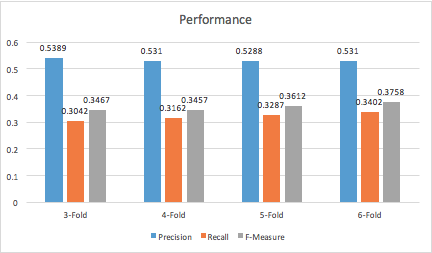
\includegraphics[width=\linewidth]{Performance1.png}
  \caption{Performance measured over different number of folds in k-fold validation}
  \label{fig:Performance1}
\end{figure}



From the results from the classifier, an analysis on the annotated data was made by studying the false positives and false negatives generated by the model. False positive is a result that indicates that a given condition has been satisfied, when it actually has not been satisfied.

The figures \ref{fig:Performance1} and \ref{fig:Performance2} are calculated using the following formulae

\begin{equation}
False Positive_k = (\sum_{i = 1}^{k} FP_i)/k
\end{equation}

\begin{equation}
True Positive_k = (\sum_{i = 1}^{k} TP_i)/k
\end{equation}

\begin{equation}
False Negative_k = (\sum_{i = 1}^{k} FN_i)/k
\end{equation}

where $False-Positive_k$ is the average number of tokens falsely recognized as API while doing $k$ fold cross validation and $FP_i$ is the number of tokens falsely recognized as API calls in the $i^{th} iteration$ among the $k$ iterations in the cross validation process. Similarly, the values of $True-Positive_k$ and $False-Negative_k$ have been calculated.

\subsection{False Positive}

\begin{center}
\begin{tabular}{ |c|c|c|c| } 
\hline
API Token & Predicted Tag & Annotated Tag \\
\hline
{AjaxControlToolkit.dll} & B-API & O \\ 
E6550 & B-API & O \\ 
Core2 & B-API & O \\ 
Dr & B-API & O \\
\hline
\end{tabular}
\end{center}

Based on the annotation and results, it can be inferred that since the tokens come under the definition of an API, the model misclassified them as their similarity to an API is high.

False negative on the other hand is when a test result indicates that a condition failed, while it actually was successful. In these following cases, the data was annotated as API but not recognized by the model. 
\begin{figure}
\centering
  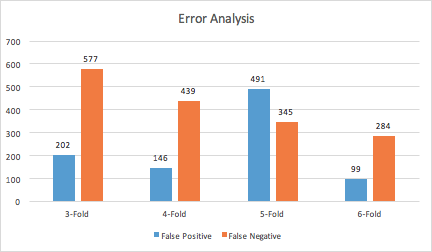
\includegraphics[width=\linewidth]{Performance2.png}
  \caption{Error Analysis measured over different number of folds in k-fold validation}
  \label{fig:Performance2}
\end{figure}

\subsection{False Negative}

\begin{center}
\begin{tabular}{ |c|c|c|c| } 
\hline
API Token & Predicted Tag & Annotated Tag \\
\hline
{this.Opacity} & O & B-API \\ 
{innerHTML} & O & B-API \\ 
check\char`_for\char`_recent\char`_keystrokes & O & B-API \\
$($ & O & I-API \\
$)$ & O & I-API \\
$CallMySproc$ & O & B-API \\
$($ & O & I-API \\
$)$ & O & I-API \\
\hline
\end{tabular}
\end{center}

In order to improve the model to identify these cases, more features must be used to train the data, and the dataset used must contain a larger pool of APIs in order to cover all cases.

\subsubsection{Ensembles Model}
Using a k-fold validation process we have analysed that training different sets of data with NER model with different parameters/training data can result in improved accuracy. Extending this information to better improve the precision, recall and the F-measure values of the model, an ensemble system is probably a better methodology for the same.

In an ensemble, model, the similarity and the differences among the data is better represented by training specific models for sets of training data which are similar and this similarity can be potentially identified by an unsupervised learning method such as $k-means$ clustering. The test data is then passes through all the training models and finally the mode of the result is calculated which leads to the predicted output for validation and testing.

\section{Application}
In real world scenario, the applications of an API recognition tool are plenty. API’s are so widely used by programmers, by making development more efficient and scalable. By implementing modularity, they facilitate the construction of large software programs and systems due to the decomposition of components into smaller pieces. However, since the data set for APIs is so large, it makes the process of accessing the desired API arduous and challenging. To overcome this obstacle, the following applications of the tools are discussed. 

\begin{description}
\item[1.]Chrome Plugin
\item[2.]Search prediction
\item[3.]Language Trend Prediction
\item[4.]Performance analysis of similar APIs
\end{description}

\subsubsection{Chrome Plugin}
Most developers come across useful APIs through websites such as stack overflow. This tool can be utilized to analyze the text of a particular webpage that the user is browsing, and based on the APIs mentioned on the webpage, the Chrome plugin can supply links for the download of associated packages and documentation. This would save the user time in searching for the source of the API. 

\subsubsection{Search prediction}
Search engines are moving towards contextual understanding. While it still remains a distant future for contextual search engine, there are integrations that already make the user experience more effective. For example, Google scans user emails for information like flight bookings. Based on this context, it provides various insights such as flight schedules and status, estimated time of travel to the airport, etc. This concept can be extended towards development. With the API recognition tool providing the necessary context, search results can be optimized for users based on their previous searches to provide significant posts relevant to the task of the User. This would make search a more time and cost effective task, and more resourceful.

\subsubsection{Language Trend Prediction}
Programming languages have been evolving over the years. In addition, the trends associated with the different languages have been tremendously changing. By feeding the information from the API recognition tool for the various languages, we can analyze the varying trends of different programming languages and understand how they are currently evolving. This can be further extended to examine the advancements in technology pertaining to software. APIs functionalities are widespread and continuously progressing. This can be utilized to discover the direction towards which new APIs would be moving. 

\subsubsection{Performance Analysis}
Efficient coding has become a necessity. Building large systems that are efficient enough to conserve space and time has become the new goal. Even Start-ups providing optimization solutions are emerging. The API recognition tool can also be used for a similar purpose. In the real world, there are multiple softwares and APIs that perform similar functionalities. The tool can be used to create a reference to the performance of a particular API and compare the space and time complexity of different APIs to find the optimized solution for the problem at hand. 

\section{Conclusion \& Future Works}
The API recognition problem is a gap in the market that developers are trying to fulfill and this project is an effort towards achieving that goal. This method has a vast potential upside and a minimal downside, in implementing a real world solution. The applications for the model are impeccable and help in eliminating this gap. Our extensive analysis of the NER model in the usage of API token recognition has yielded the fact that utilizing Named Entity Recognition has widespread applications in our day to day life. Using NER, a simple yet classic API recognition tool can be built that has many benefits and high relevance. The model can be further improved by using a larger dataset with more precise annotations of API mentions to improve the training of the model. Additionally, we could improve Named Entity Recognition by detecting Non-Standard Words(NSW). This is done by analyzing if a word is Out of Vocabulary (OOV) using the information available in the dictionary, and using the normalization results of these words to determine if they are NSW \cite{liimproving}. Also, as mentioned in the error analysis, using an ensemble of classifiers could improve the model by generating more certain, precise and accurate system results.

\bibliographystyle{abbrv}
\bibliography{sigproc}  % sigproc.bib is the name of the Bibliography in this case
\end{document}
